\documentclass{article}
\usepackage{amsmath}
\usepackage{setspace}
\usepackage{tasks}
\usepackage{graphicx}
\usepackage{listings}
\newcommand{\norm}[1]{\lVert#1\rVert}
\renewcommand{\vec}[1]{\textbf{#1}}
%\renewcommand{\thechoice}{\Alph{choice}}
\begin{document}
\onehalfspacing
\begin{center}
	\section*{\textbf{Class 12}}
	\subsection*{Chapter 10 - Vector Algebra}
\end{center}
The following problem is question 17 from exercise 10.5

\begin{enumerate}
	\item Let $\vec{a}$ and $\vec{b}$ be two unit vectors and $\theta$ is the angle between them. Then $\vec{a}+\vec{b}$ is a unit vector if
		\begin{tasks}(4)
			\task $\theta = \frac{\pi}{4}$
			\task $\theta = \frac{\pi}{3}$
			\task $\theta = \frac{\pi}{2}$
			\task $\theta = \frac{2\pi}{3}$
			\end{tasks}
			
\end{enumerate}
	\textbf{Solution:}
\\
Given,
\begin{align}
	\norm{\vec{a}}=\norm{\vec{b}}=1\label{eq:1}
	\\
	\norm{\vec{a}+\vec{b}}=1\label{eq:2}
\end{align}
Squaring both sides of \eqref{eq:2}  , we get
\begin{align}
	\norm{\vec{a}+\vec{b}}^2=1^2
\\	
	\implies \norm{\vec{a}}^2 + \norm{\vec{b}}^2 + 2\vec{a}^{\top}\vec{b} = 1\label{eq:3}	
\end{align}
Substituting \eqref{eq:1} in \eqref{eq:3}, we get
\\
\begin{align}
	\implies 1+1+2(\norm{\vec{a}}\norm{\vec{b}}\cos{\theta})=1
	\\
	\implies 2+2(\norm{\vec{a}}\norm{\vec{b}}\cos{\theta})=1
        \\
	\implies 2(\norm{\vec{a}}\norm{\vec{b}}\cos{\theta})=-1
	\\
	\implies (\norm{\vec{a}}\norm{\vec{b}}\cos{\theta})=\frac{-1}{2}\label{eq:4}
\end{align}
Subtituting \eqref{eq:1} in \eqref{eq:4}, we get
\begin{align}
	\implies \cos{\theta}=\frac{-1}{2}
	\\
	\implies \theta=\frac{2\pi}{3}
\end{align}
\begin{figure}[!h]
	\begin{center}
	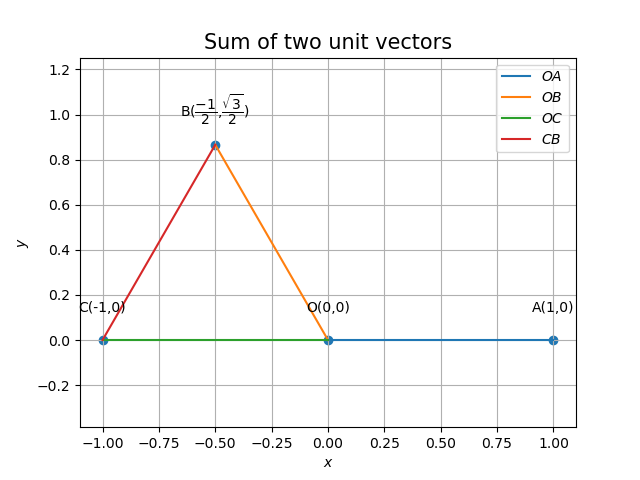
\includegraphics[width=\columnwidth]{codes/Python/figs/fig.png}
	\end{center}
	\caption{$\vec{OA}$ and $\vec{CO}$ is $\vec{a}$ and $\vec{OB}$ is $\vec{b}$ and $\vec{CB}$ is $\vec{a+b}$}
	\label{fig:Fig1}
\end{figure}
\end{document}

